\documentclass[a4paper]{article}
\usepackage{listings}
\usepackage{xcolor}
\usepackage {fontspec}
\usepackage{fancyhdr}
\pagestyle{fancy}
\setromanfont{Lantinghei SC Extralight}
\setmonofont{Courier New}
\XeTeXlinebreaklocale ``zh''
\XeTeXlinebreakskip = 0pt plus 1pt
\textheight = 650pt
\lstset{
	%行号
   numbers=left,
  %背景框
   framexleftmargin=10mm,
   frame=none,
   %背景色
   %backgroundcolor=\color[rgb]{1,1,0.76},
   backgroundcolor=\color[RGB]{245,245,244},
   %样式
   keywordstyle=\bf\color{blue},
   identifierstyle=\bf,
   numberstyle=\tiny,
   numberstyle=\color[RGB]{0,192,192},
   commentstyle=\it\color[RGB]{0,96,96},
   stringstyle=\rmfamily\slshape\color[RGB]{128,0,0},
   %显示空格
   showstringspaces=false
 }

\begin{document}
\title{实验报告 实验七}
\author{姓名:王钦\quad 学号:13349112\quad 班级:计科二班}
\date{}

\maketitle
\section*{ 实验目的}
\hangindent=4em \hangafter=-10{
  1. 学习进程模型知识,掌握进程模型的实现方法。\\
  2. 利用时钟中断,设计时钟中断处理进行进程交替执行\\
  3. 扩展MyOS,实现多进程模型的原型操作系统\\
}
\section*{ 实验内容}
\hangindent=4em \hangafter=-10{
在实验五或更后的原型基础上,进化你的原型操作系统,原型保留原有特征的基础上,设计满足下列要求的新原型操作系统:\\
(1)实现控制的基本原语do\_fork()、 do\_wait()、do\_exit()、blocked()和wakeup()。\\
(2)内核实现三系统调用fork()、 wait()和exit() ,并在c库中封装相关的系统调用.\\
(3)编写一个c语言程序,实现多进程合作的应用程序。\\
多进程合作的应用程序可以在下面的基础上完成:由父进程生成一个字符串,交给子进程统计其中字母的个数,然后在父进程中输出这一统计结果。\\
参考程序如下:\\
{\scriptsize
	\begin{lstlisting}[language={C}]
char str[80]="129djwqhdsajd128dw9i39ie93i8494urjoiew98kdkd";
int LetterNr=0;
void main() {
   int pid;
   char ch;
   pid=fork();
   if (pid==-1) printf("error in fork!");
   if (pid)  {
	 ch=wait(); 
	 printf("LetterNr=");
	 ntos(LetterNr);
   }
   Else {
	 CountLetter(str);
	 exit(0);
   }
}
\end{lstlisting}}
编译连接你编写的用户程序,产生一个com文件,放进程原型操作系统映像盘中。\\

}

\section*{ 实验平台}
\hangindent=4em \hangafter=-10{
  xxd+dd+gcc+ld+nasm+Linux+vim\\
}

\section*{ 算法流程图}
\hangindent=4em \hangafter=-10{
  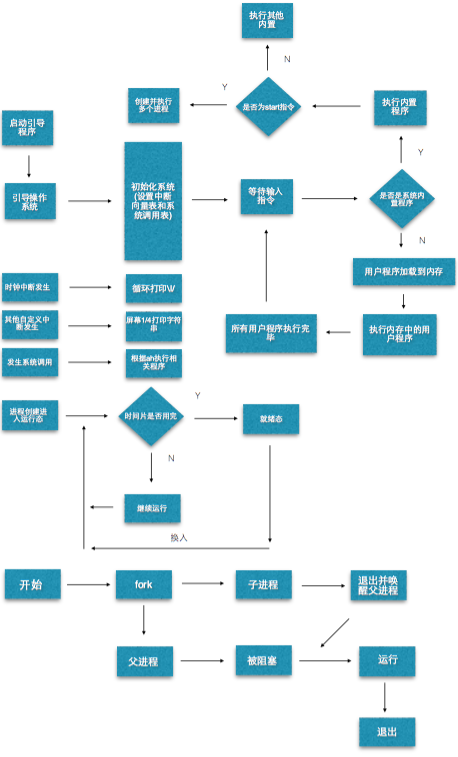
\includegraphics[scale=0.6]{Illustrations/flow.png}
}

\section*{ 功能一览}
\hangindent=4em \hangafter=-50{
	{\large 1. 系统内置功能:}\\
		\indent \verb| terminal|,装载内核shell,为用户提供一个与操作系统交互的工具,开机后自动进入,以下所有功能都在terminal中交互\\
		\indent	\verb| date|, 显示当前日期\\
		\indent \verb| time|, 显示当前时间\\
		\indent \verb| asc|, 显示一个字符的asc码\\
		\indent \verb| clear|, 清除当前屏幕所有字符,刷新屏幕\\
		\indent \verb| help|, 显示系统帮助信息\\
		\indent \verb| man |, 显示内置函数的帮助信息,比如\verb| man date |,显示date的相关帮助\\
		\indent \verb| python |, python 扩展,类似python命令行工具,可以使用这个工具输入计算表达式返回计算结果,目前只支持加法减法\\
		\indent \verb| start|, 开始创建并执行四个进程并且每秒18.2次的调度,分别在屏幕\verb|1/4|处打印一些个性化信息( 不同配置的虚拟机动画速度不一样,建议使用vmware测试)\\\\
	{\large 2. 用户程序:}\\
		\indent \verb| run |,软盘中含有两个用户程序,输入\verb|run 12|,可分别执行两个用户程序,当然也可以通过改变执行序列来改变执行的顺序\\\\
	{\large 3. 自定义中断:}\\
		\indent 时钟中断:通过PTR每秒发出18.2次的信号来从8592芯片的RT0引脚发出终端号\verb|int 08h|来触发的用户时钟软中断\verb| int 1ch|,实现在\verb|terminal|的右下角
	  一个横杠在转动.\\
		\indent 另外有自定义中断\verb|int 33h,int 34h,int 35h,int 36h|分别在屏幕四分之一的位置打印个性化信息\\\\
	{\large 4. 进程调度:}\\
		\indent 软盘中共存放了用于展示进程调度的六个应用程序,其中一个应用程序为监听用户键盘事件然后退出多进程调度状态回到\verb| terminal|每个应用程序分别代表一个进程。开启装载进程并进行进程调度由\verb|1|中系统内置功能的\verb| start|指令激活。\\
		\\
	{\large 5. 进程\verb|fork,wait,exit|:}\\
		\indent 这个功能也是本次实验要求实现的,具体使用在第六个进程中,执行\verb|start|后即可看到包括第六个进程在内全部进程执行的结果。
}

\section*{ 实验步骤及效果图}
\hangindent=4em \hangafter=-50{
1. 编辑修改ASM 文件,和C文件	\\\\
2. 使用make命令配合\verb|makefile|文件进行编译	\\\\
3. 运行\verb|bochs or vmware|虚拟机进行测试,输入\verb|man start|,查看此条指令的说明\\\\
{\center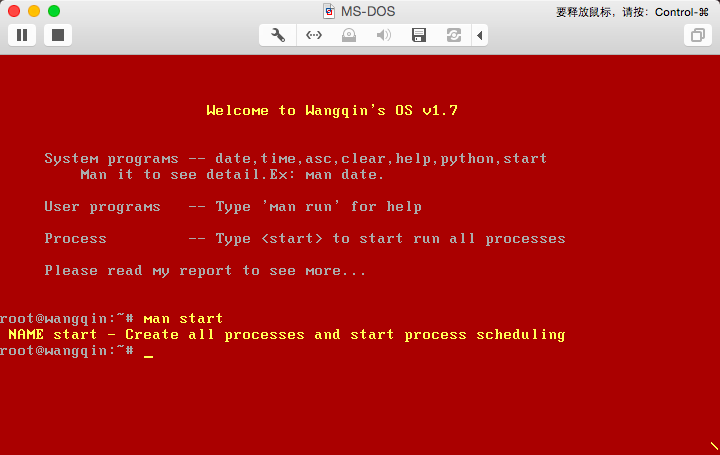
\includegraphics[scale=0.45]{Illustrations/man_start.png}}\\\\
4. 输入\verb|start| 指令测试本次实验要求实现的功能
{\center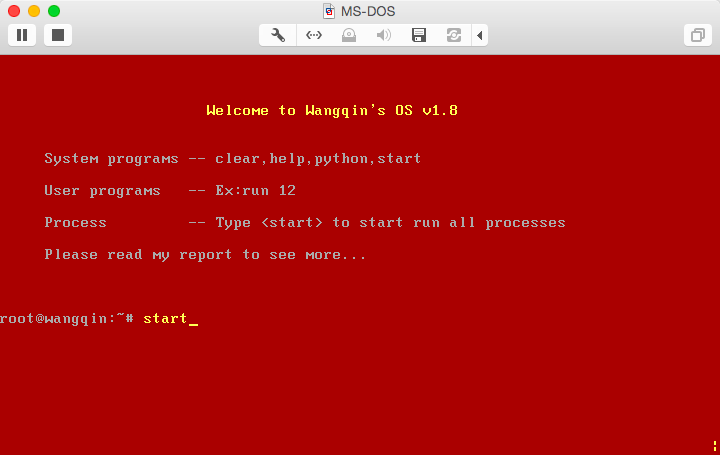
\includegraphics[scale=0.45]{Illustrations/start.png}}\\\\
5. 执行\verb| start|后开始执行的进程包括四个分别在\verb|1/4|屏幕打印个性信息的进程和一个监听任意按键退出的进程最后一个就是本次实验要测试的含有fork等函数的c语言进程,一共6个进程,
下面是这个c进程的详细代码\\\\
{\scriptsize
	\begin{lstlisting}[language={C}]
process_counter.c

#include "muti_process.h"

char str[ 80] = "129djwqhdsajd128dw9i39ie93i8494urjoiew98kdkd";
int LetterNr = 0;
void main() {
    __asm__( "sti");
    int pid;
    char ch;
    printf( "\r\nBefore fork \r\n");
    printf( "fork start..");
    pid = fork();
    if ( pid == -1) printf( "error in fork!\0");
    if ( pid){
        printf( "\r\nFather process:after fork pid is ");
        printInt( pid);
        printf( "\r\nFather process:running...");
        printf( "\r\nFather process:blocked \r\n\r\n");

        ch = wait();
        printf( "\r\nFather process:running...");
        printf( "\n\rFather process:LetterNr=");
        ntos( LetterNr);
        printf( "\r\nFather process:exit");
        exit(0);
    }
    else{
        printf( "\r\nSub process:after fork pid is ");
        printInt( pid);
        printf( "\r\nSub process:running...");

        CountLetter( str);
        printf( "\r\nSub process:exit\r\n\r\n");
        exit( 0);
    }
}
	\end{lstlisting}
}



6. 下图就是刚执行后的效果,6个进程开始执行并调度
{\center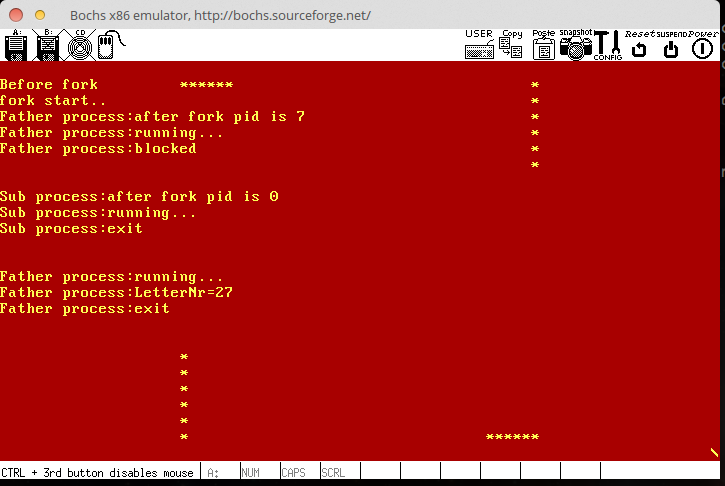
\includegraphics[scale=0.45]{Illustrations/fork_begin.png}}\\\\
{\center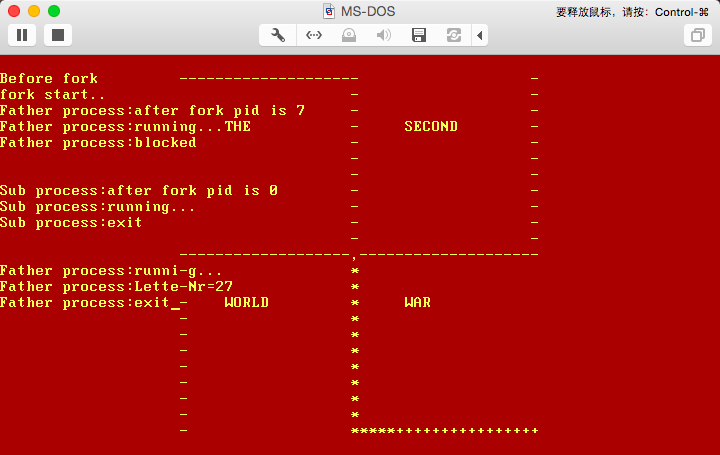
\includegraphics[scale=0.45]{illustrations/fork_done.png}}\\\\
7. 下面具体解释一下执行的详细过程,可以参照第5步贴的代码,绿色框内是执行fork之前输出的字符串,黄色框代表fork后父进程输出的代码,紫色是fork后子进程输出的。
可以看到fork完之后父进程运行了一段时间后被阻塞,然后子进程继续运行直到退出并唤醒父进程。父进程再次执行并把子进程执行\verb|countletter|的结果打印出来,最后父进程退出
\\\\
{\center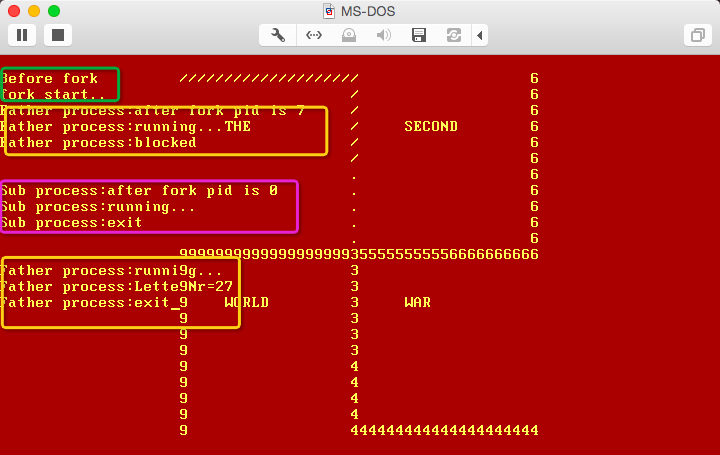
\includegraphics[scale=0.45]{illustrations/intro.png}}\\\\
8. 再执行的任何时间都可以按下任意按键退出模拟多进程调度的程序回到\verb|terminal|。\\\\
{\center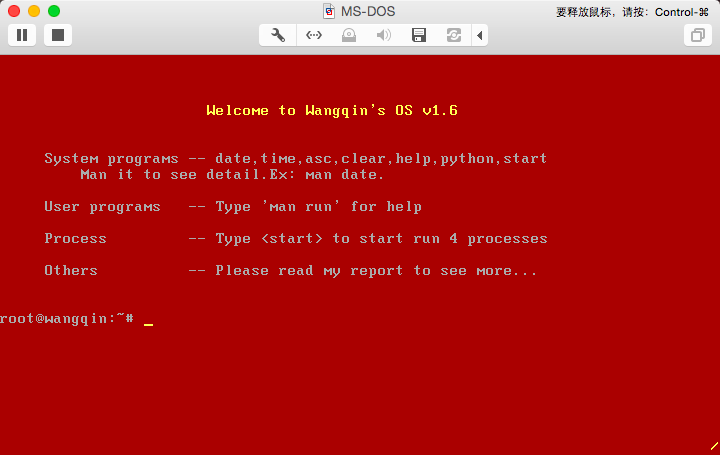
\includegraphics[scale=0.45]{illustrations/back.png}}\\\\







\section*{ 内存和软盘存储管理}
\hangindent=4em \hangafter=-50{
1. 引导程序加载到内存0x7c00处运行\\
2. 引导程序将操作系统加载到0x7e00处运行\\
3. 操作系统讲用户程序加载到0x1000处运行\\
4. 软盘第0个柱面的第一个扇区存储操作系统引导程序\\
5. 软盘第0个柱面剩下所有扇区2~36扇区存储操作系统内核\\
6. 软盘第\verb|1,2,3,4,5,6|柱面分别存储六个进程代码\\
7. 软盘第\verb|7,8|柱面分别存储两个用户程序的程序代码\\\\
{\large 栈结构}\\
	\indent 内核栈:从内存的\verb| 0xffff|开始向下扩展\\
	\indent 用户栈:从内存的\verb| 0x1000|开始向下扩展\\
	\indent 进程栈:第i个进程对应的进程栈从内存的\verb| i*0x800|开始向下扩展\\\\
更多细节信息请阅读我的Makefile文件
}
\section*{ 系统目录架构}
\hangindent=4em \hangafter=-50{
{\scriptsize
  \setmonofont{Lantinghei SC Extralight}
\begin{verbatim}
.
├── Makefile						makefile 文件
├── README
├── bochsrc
├── boot.asm						引导程序
├── disk.img
├── kernel                          目录中存放内核相关代码
│   ├── os.asm						主要为os.c提供函数实现.
│   ├── os.c                        为内核主要控制模块
│   ├── os.h                        主要为os.c提供函数实现.
│   ├── os_syscall.asm
│   ├── osclib.c                    为osclib.c提供更底层的函数封装
│   ├── oslib.asm                   初始化系统调用和设置系统调用相关模块
│   ├── pcb.h
│   ├── process.c                   进程调度创建相关代码
│   ├── terminal.c                  装载shell的工具
│   └── terminal.h
├── muti_process.h                  fork,wait,wakeup,printf等声明实现
├── osclib_share.c                  内核和用户的共享库(使用户程序体积减少)。
├── oslib_share.asm                 内核和用户的共享库(使用户程序体积减少)。
├── process1.asm                    第一个进程
├── process2.asm                    第二个进程
├── process3.asm                    ..
├── process4.asm                    ..
├── process_counter.c				统计字母个数的进程
├── process_wait_key.asm            监听退出进程
├── python_extension.c              Python扩展
├── report                          实验报告目录
│   ├── Illustrations               插图
│   │   ├── back.png
│   │   ├── flow.png
│   │   ├── fork_begin.png
│   │   ├── fork_done.png
│   │   ├── intro.png
│   │   ├── man_start.png
│   │   └── start.png
│   ├── report.aux
│   ├── report.log
│   ├── report.pdf
│   ├── report.tex					latex源码
│   └── tree
├── snapshot.txt
├── usr1.asm						用户代码
└── usr2.asm

1 directory, 28 files
\end{verbatim}}
}

\setmonofont{Courier New}

\section*{ 主要函数模块}
\hangindent=4em \hangafter=-50{
	1. \verb|process.c: do_fork| 函数模块,这个模块是本次试验要求实现fork的核心代码,注意的地方就是要在复制父进程的上下文tss之前要保存一下父进程现在的状态到pcb,另外就是串操作复制父进程栈的时候要注意寻址方式\verb| ss*16+sp|,\verb| w_is_r|表示当前正在运行进程在数组中的\verb| index|
{\scriptsize\begin{lstlisting}[language={C}]

extern void restore_flags();
short int sub_stack,fa_stack;
void do_fork(){
    process_num++;
	//add index for new sub process
    PCB_queue[ process_num].f_pid = w_is_r;
	//sub -> father
    PCB_queue[ process_num].process_id = process_num;
	//sub->pid = new index
    //copy_fa_Tss

    update_fa();				//save father regsiters to pcb
    restore_flags();    //to fix some stack bug
    __asm__("pop %cx");
    // update fa end
    PCB_queue[ process_num].tss = PCB_queue[ w_is_r].tss;
	//sub.tss=father.tss
    PCB_queue[ process_num].tss.SP = _sp + 0x1000;
	//sub.stack_pointer = father.stack_pointer+0x1000
    PCB_queue[ process_num].tss.AX = 0;
	//father process return pid is 0
    PCB_queue[ process_num].tss.Stack_END=PCB_queue[ w_is_r].tss.Stack_END+0x1000;
	//ss

    sub_stack = (PCB_queue[ process_num].tss.Stack_END-0x200)/16;
	//sub_stack_segmentaddress-> find address   ss*16+sp
    fa_stack = (PCB_queue[ w_is_r].tss.Stack_END-0x200)/16;
	//father_stack_segment_addr
    __asm__("mov $0x104,%cx");		//movsw length
    copy_stack();			//movsw
    __asm__("pop %cx");

    PCB_queue[ process_num].process_status = READY;
	//sub process into READY queue

    restore_ax_pid();
	// sub process return pid is self pid
    __asm__("pop %bx");

    __asm__("pop %bx");
    __asm__("pop %bx");
    __asm__("pop %bx");
    __asm__("jmp *%bx");
	//end of syscall
}

 \end{lstlisting}}
	2. \verb| copy_stack|模块,使用串操作复制父进程栈的内容到子进程栈
{\scriptsize
	\begin{lstlisting}[language={C}]
	global copy_stack
	extern sub_stack,fa_stack
	copy_stack:
	push ax
	push es
	push ds
	push di
	push si
	push cx
	mov ax,[ sub_stack]
	mov es,ax
	mov edi,4

	mov byte [es:di],0x12   ;3df0

	mov ax,[ fa_stack]
	mov ds,ax
	mov esi,4
	cld
	rep movsw           ;ds:si  ->  es:di
	pop cx
	pop si
	pop di
	pop ds
	pop es
	pop ax
	ret
	\end{lstlisting}}
	3. \verb|do_wait|和\verb| do_exit|模块,这两个模块实现起来就比较简单,改变一下进程的状态就好了
{\scriptsize
	\begin{lstlisting}[language={C}]
	global copy_stack
void do_wait(){
    PCB_queue[ w_is_r].process_status = BLOCK;
    __asm__("int $0x1c");
    __asm__("pop %ax");
    __asm__("pop %ax");
    __asm__("pop %ax");
    __asm__("jmp *%ax");
}
void do_exit(){
    PCB_queue[ w_is_r].process_status = DONE;
    PCB_queue[ PCB_queue[ w_is_r].f_pid].process_status = READY;
    __asm__("int $0x1c");
    __asm__("pop %ax");
    __asm__("pop %ax");
    __asm__("pop %ax");
    __asm__("jmp *%ax");
}

\end{lstlisting}}
4. 进程调度模块, 这个模块对上一个实验中的\verb| schedule|进行了修改,主要修改是调度的时候调整了对不同进程状态的筛选,例如一个进程要被送上cpu的时候必须是就绪态等。
{\scriptsize
	\begin{lstlisting}[language={C}]
int fin_times = 0;
void schedule(){
    saveall_reg();          //hurry not inclue sp
    __asm__("pop %cx");
    __asm__("pop %eax");    //junk

    if( PCB_queue[ w_is_r].process_status == RUNNING){
        PCB_queue[ w_is_r].process_status = READY;
    }
    while(1){
        if( w_is_r == 0)
            nw_is_r = start_process_num;
        else
            nw_is_r = w_is_r + 1;

        if( nw_is_r > process_num){
            nw_is_r = start_process_num;
        }
        if( PCB_queue[ nw_is_r].process_status == READY) break;
        w_is_r = nw_is_r;
    }

    PCB_queue[ nw_is_r].process_status = RUNNING;

    saveToqueue();          //code order don't change

    //----------------set ip cs flag--------
    __asm__("pop %ax");
    __asm__("pop %bx");
    __asm__("pop %cx");

    saveall_reg_seg();      //include sp
    __asm__("pop %cx");

    if( _di == 0x1234){
        isProcessRun = 0;           //shut down process
        nw_is_r = 0;
        process_num --;
        backto_os();
    }else{
        isProcessRun = 1;
    }


    PCB_queue[ w_is_r].tss.SP = _sp;
    PCB_queue[ w_is_r].tss.IP = _ip;
    PCB_queue[ w_is_r].tss.CS = _cs;
    PCB_queue[ w_is_r].tss.Flags = _flags;

    //-----------------end------------------
    _ip = PCB_queue[ nw_is_r].tss.IP;
    _cs = PCB_queue[ nw_is_r].tss.CS;
    _flags = PCB_queue[ nw_is_r].tss.Flags;
    _sp = PCB_queue[ nw_is_r].tss.SP;

    restore_reg_seg();      //include sp
    __asm__("pop %cx");

    queueTodata();      // ax bx cx...

    w_is_r = nw_is_r;           //change now running process
    restore_reg();
    __asm__(" pop %di");        //don't use di in any process is dangerous

    __asm__(" jmp schedule_end");
    while(1);
}

	\end{lstlisting}
  }
  5. \verb| muti_process.h|中的\verb| fork,wait,exit|,分别对应系统功能号为\verb| 6,7,8|的系统调用.
  {\scriptsize \begin{lstlisting}[language={C}]

extern char return_ax_Tpid();
char pid;
char fork(){
    __asm__("cli");
    __asm__("mov $6,%ah");
    __asm__("int $0x80");

    pid = return_ax_Tpid();
    __asm__("pop %cx");
    __asm__("sti");
    return pid;
}


char wait(){
    __asm__("cli");
    __asm__("mov $7,%ah");
    __asm__("int $0x80");
    __asm__("sti");
    return pid;
}

void exit( char x){
    __asm__("cli");
    __asm__("mov $8,%ah");
    __asm__("int $0x80");
    __asm__("sti");
    while(1);
}

	\end{lstlisting}}
  6. \verb| Countletter| 函数实现,这个比较简单没什么好说的就是从给出的一串字符串中统计里面字母的个数
  {\scriptsize \begin{lstlisting}[language={C}]
extern int LetterNr;
void inline CountLetter( char *str){
    char i;
    for (i = 0;i<80;i++){
        if( str[ i] <='z' && str[ i] >='a'){
            LetterNr++;
        }
    }
}
	\end{lstlisting}}

}
\section*{ 实验心得及仍需改进之处}
\hangindent=4em \hangafter=-50{
	{\large 实验心得:}\\\\
	\indent 本次实验过程还算轻松,没有遇到一些难以解决的bug,不过也是有一些地方卡了很久,比如说上次实验的进程栈栈指针是从0开始隔0x1000一个,这次因为进程比较多,fork完后是7个,又由于前面五个进程根本用不到这么大的栈所以改成了隔\verb| 0x800|为一个进程栈,我当时写代码的时候以为\verb|0x1000/2 = 0x500|,然后设置栈指针的时候设置为\verb| 0x500*i|,后来调了大半天发现\verb| 0x1000/2 = 0x800|并不是\verb|0x500|,细节上稍微一不注意,这种低级错误就会发生,写汇编的时候纪要抛弃原来十进制的思维方式。\\
	\indent 另外就是要注意fork时复制之前一定要保存一下父进程的状态到pcb,并不是只有到被调度的时候才保存,fork的时候如果没有更新pcb就复制父进程的pcb,显然不能复制到父进程最新的pcb,导致fork出错。\\
	\indent \verb|do_wait,do_exit |的时候要注意, 改变完进程状态后马上手动触发下\verb| 0x1c| 时钟中断,将本进程根据进程状态进行处理。否则并不能起到马上改变进程状态的作用,因为要等待下一次时钟中断发生.\\\\
\\
	{\large 实验仍需改进之处:}\\\\
	\indent 仍需完善细节,比如说\verb|python|的命令行工具加入乘法,除法完全是几行代码的问题\\
	\indent 可以考虑将用户程序做成\verb|elf|格式,动态链接系统的代码库。目前的情况是用户程序自己带着一份和操作系统一样的代码库,分别联合编译\\
	\indent 精简操作系统代码,减少冗余代码\\
	\indent 增加文件系统功能\\
	\indent 调度算法和进程控制模块的存储有待优化,使用链表来实现pcb\\
	\indent 如果时间片很小,父进程在执行到 wait 之前就被调度,接下来子进程完成了整个程序的执行,然后exit,然后父进程重新开始执行,那么此时父进程执行了 wait,变成阻塞态,接下来一直无法运行,也没有子进程来更改父进程的状态,父进程就会无限等待下去。所以,这个问题应该要靠使用信号量的PV操作来解决\\
}
\end{document}
